\section{Background Estimation}
\label{sec:backgroundestimation}

\subsection{Data-Driven Background Estimation Using the \texorpdfstring{\twoxtwod}{2x2D} Sidebands}


\subsubsection{Description of the \twoxtwod\ Sideband Method}
\label{subsec:2x2ddescriptionmethod}

The double-two-dimensional (\twoxtwod) sidebands method \cite{STDM-2011-05} is a standard method for estimating the composition of the background in diphoton events. The same procedure is employed as in the two previous measurements at 13 \TeV \cite{HIGG-2019-13} and 13.6 \TeV (31.4 \ifb) \cite{HIGG-2022-12}. The procedure is described in detail in the Internal Notes \cite{HIGG-2019-13-INT1,HIGG-2022-10-INT1}.

The main sources of background are the non-resonant production of prompt and isolated diphotons ($\gamma \gamma$) and the $\gamma j$ and $jj$ processes where one or two hadronic jets are misidentified as photons. 

In the \twoxtwod\ method, the identification and isolation requirements for the photons are loosened. Only events passing the \texttt{LoosePrime3} working point are considered in the nominal result. This criterion is defined by relaxing three strip variables ($\omega_{s3}$, $F_\mathrm{side}$ and $\Delta E$) with respect to the Tight criterion. Details of the photon identification variables are given in \cite{PERF-2017-02}.

Systematic uncertainties are evaluated by comparing the loosened identification pre-selection at the \texttt{LoosePrime3} working point to the alternative definitions \texttt{LoosePrime2}, \texttt{LoosePrime4} and \texttt{LoosePrime5}. Both \texttt{LoosePrime4} and \texttt{LoosePrime5} require an additional cut on the variable $E_\mathrm{ratio}$ and, in addition, \texttt{LoosePrime5} imposes a cut on $w_\mathrm{s\,tot}$. The \texttt{LoosePrime2} working point relaxes than the nominal criteria by not requiring a cut on $\Delta E$. \texttt{LoosePrime4} and \texttt{LoosePrime5} typically yield a higher $\gamma \gamma$ purity than \texttt{LoosePrime3}, while \texttt{LoosePrime2} yields a lower purity. The systematic uncertainty on the background yields is taken as the sum of squares of positive (negative) deviations from the nominal result obtained with the three alternative working points.

% Why three different working points?
% ALEX: What shall we do with these systematic uncertainties? Is this prescription still good? Discuss with Liza and Luis.

The events are separated into 16 orthogonal regions, defined by whether one or both photons pass or fail the nominal identification and isolation requirements. The \(\gamma\gamma\), \(\gamma j\) and \(jj\) yields after the nominal selection are obtained by solving a system of equations, given the observed yields in the 16 regions, as well as the photon identification and isolation efficiencies as estimated from MC simulation. 

The fractions contributed by the \(\gamma\gamma\), \(\gamma j\) and \(jj\) background sources after the inclusive diphoton selection are \SI{66.9}{\percent}, \SI{28.8}{\percent} and \SI{4.4}{\percent}, respectively, as shown in Table \ref{tab:2x2dinclusive202224}. 



% \subsubsection{Plots and Tables}
\subsubsection{Background Yields and Fractions}
\label{subsec:2x2dyieldsfractions}

Inclusive background yields and fractions are shown for the full 2022--2024 dataset in Table \ref{tab:2x2dinclusive202224} with the statistical and systematic uncertainties, as well as the yields and fractions for the alternative \texttt{LoosePrime} working points form which the latter have been derived. Corresponding values for the individual 2022, 2023, and 2024 data periods are shown in Tables \ref{tab:2x2dinclusive2022}--\ref{tab:2x2dinclusive2024}.

\newpage
\FloatBarrier

\begin{table}[!h]
    \centering
    \caption{Background decomposition using the \twoxtwod\ sidebands method for 2022-2024 data and \texttt{mc23a-e}.}
    \includegraphics[width=\textwidth,page=3,trim={4.2cm 24.1cm 4.2cm 3.5cm},clip]{figures/2x2d_sidebands/plots_sb_diffxsvars_20250930/table_HGam2x2DBkgDecomp_Xsection.pdf}
    \label{tab:2x2dinclusive202224}
\end{table}


\begin{table}[!h]
    \centering
    \caption{Background decomposition using the \twoxtwod\ sidebands method for 2022 data and \texttt{mc23a}.}
    \includegraphics[width=\textwidth,page=2,trim={4.85cm 24.9cm 4.85cm 3.5cm},clip]{figures/2x2d_sidebands/sb_h032_2022_debug/table_HGam2x2DBkgDecomp_Xsection_SpringPaper.pdf}
    \label{tab:2x2dinclusive2022}
\end{table}


\begin{table}[!h]
    \centering
    \caption{Background decomposition using the \twoxtwod\ sidebands method for 2023 data and \texttt{mc23d}.}
    \includegraphics[width=\textwidth,page=2,trim={4.85cm 24.9cm 4.85cm 3.5cm},clip]{figures/2x2d_sidebands/sb_h032_2023_debug/table_HGam2x2DBkgDecomp_Xsection_SpringPaper.pdf}
    \label{tab:2x2dinclusive2023}
\end{table}


\begin{table}[!h]
    \centering
    \caption{Background decomposition using the \twoxtwod\ sidebands method for 2024 data and \texttt{mc23e}.}
    \includegraphics[width=\textwidth,page=2,trim={4.6cm 24.9cm 4.6cm 3.5cm},clip]{figures/2x2d_sidebands/sb_h032_2024_debug/table_HGam2x2DBkgDecomp_Xsection_SpringPaper.pdf}
    \label{tab:2x2dinclusive2024}
\end{table}

% Plots

\newpage
\FloatBarrier

\subsubsection{Differential Plots: Background Yields}
\label{subsec:2x2dyieldsplots}

\begin{figure}[!h]
    \centering
    \includegraphics[width=0.8\textwidth]{figures/2x2d_sidebands/plots_sb_diffxsvars_20250930/plot_bkgDecomp_Inclusive_inclusive.pdf}
    \label{fig:2x2dinclusive202224}
    \caption{Inclusive background yields for 2022--2024 data (\texttt{mc23a--e}).}
\end{figure}

% \begin{figure}[!h]
%     \centering
%     \begin{subfigure}{0.45\textwidth}
%         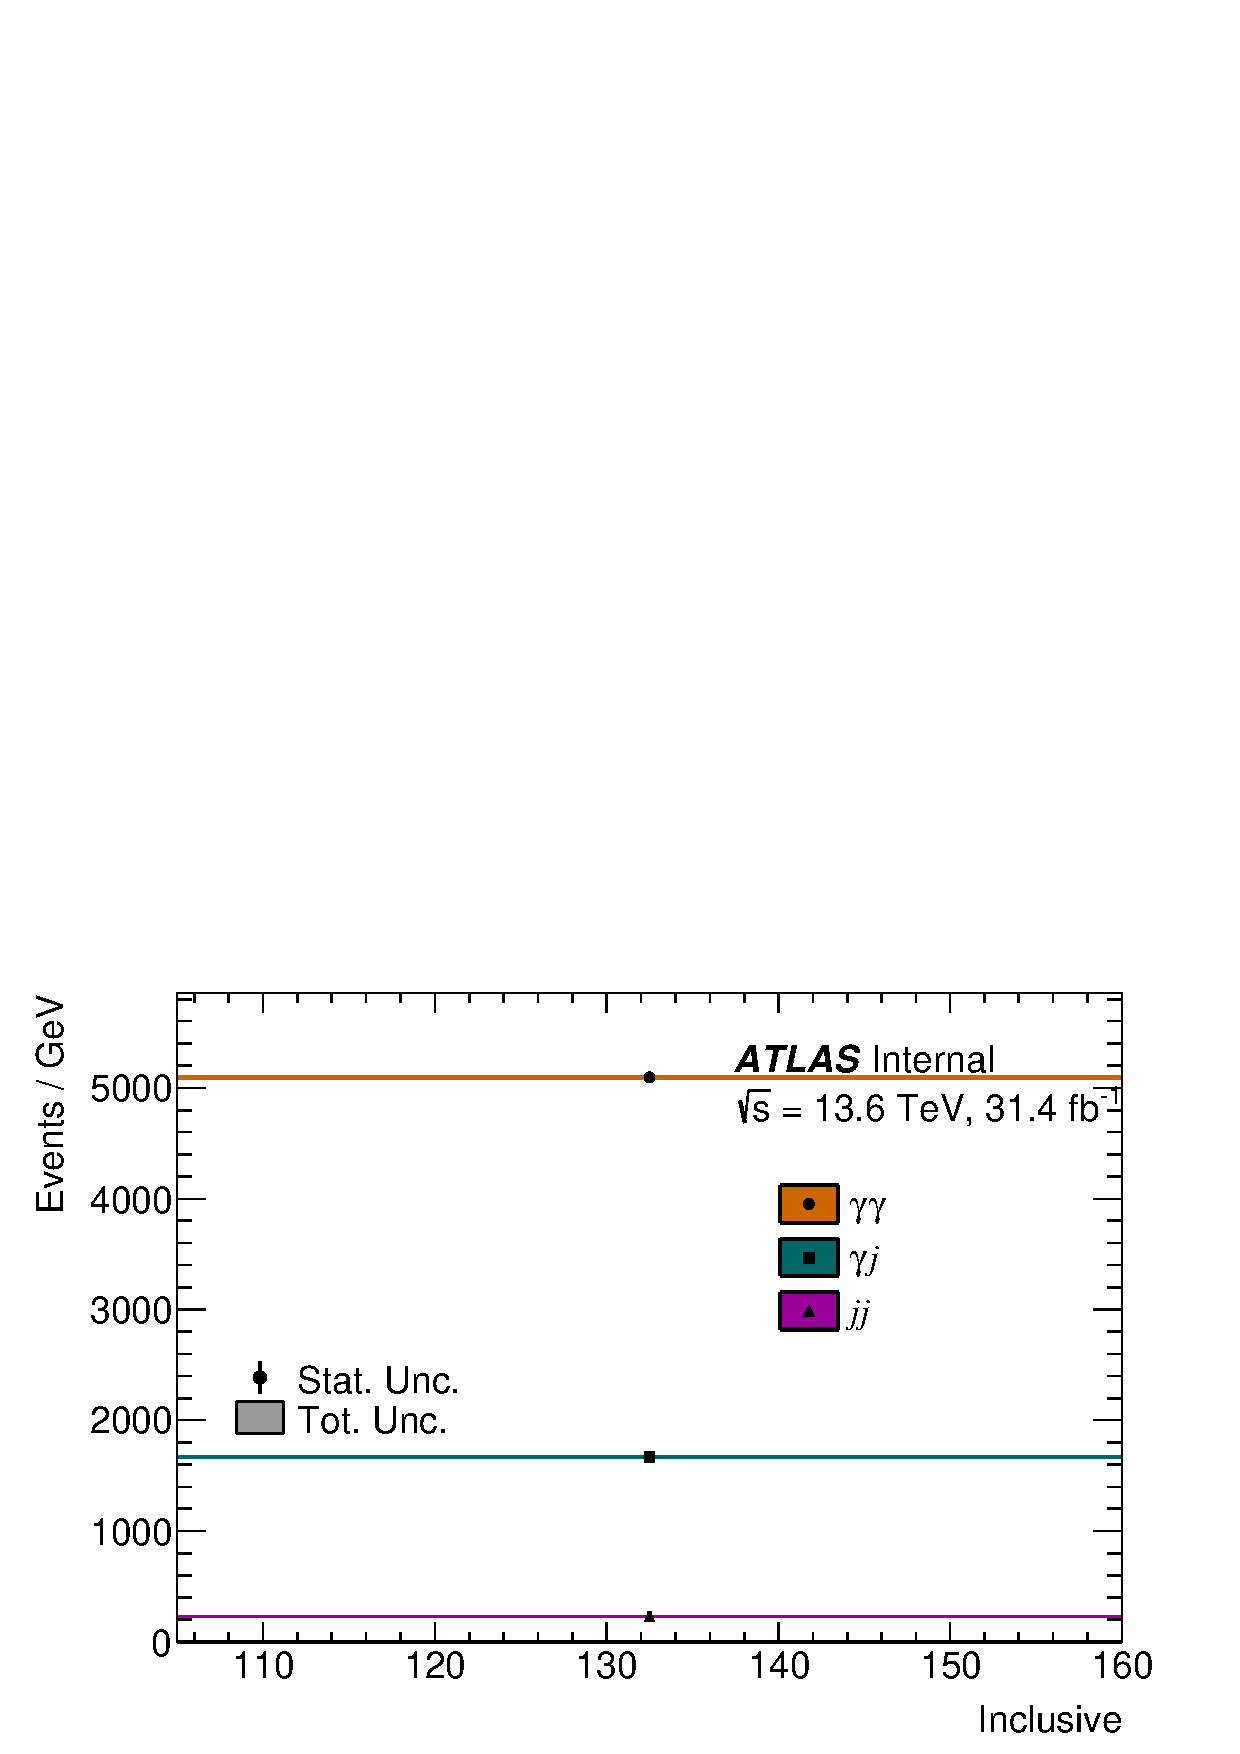
\includegraphics[width=0.8\textwidth]{figures/2x2d_sidebands/sb_h032_2022_debug/plots/plot_bkgDecomp_Inclusive_inclusive.pdf}
%         \label{fig:2x2dinclusive2022}
%     \end{subfigure}
%     \begin{subfigure}{0.45\textwidth}
%         \includegraphics[width=0.8\textwidth]{figures/2x2d_sidebands/sb_h032_2023_debug/plots/plot_bkgDecomp_Inclusive_inclusive.pdf}
%         \label{fig:2x2dinclusive2023}
%     \end{subfigure}
%     \begin{subfigure}{0.45\textwidth}
%         \includegraphics[width=0.8\textwidth]{figures/2x2d_sidebands/sb_h032_2024_debug/plots/plot_bkgDecomp_Inclusive_inclusive.pdf}
%         \label{fig:2x2dinclusive2024}
%     \end{subfigure}
%     \begin{subfigure}{0.45\textwidth}
%         \includegraphics[width=0.8\textwidth]{figures/2x2d_sidebands/plots_sb_diffxsvars_20250930/plot_bkgDecomp_Inclusive_inclusive.pdf}
%         \label{fig:2x2dinclusive2024}
%     \end{subfigure}
%     \caption{Inclusive background yields for 2022 (a), 2023 (b) and 2024 (c) data (\texttt{mc23a}, \texttt{mc23d} and \texttt{mc23e}).}
% \end{figure}

\begin{figure}[!h]
    \centering
    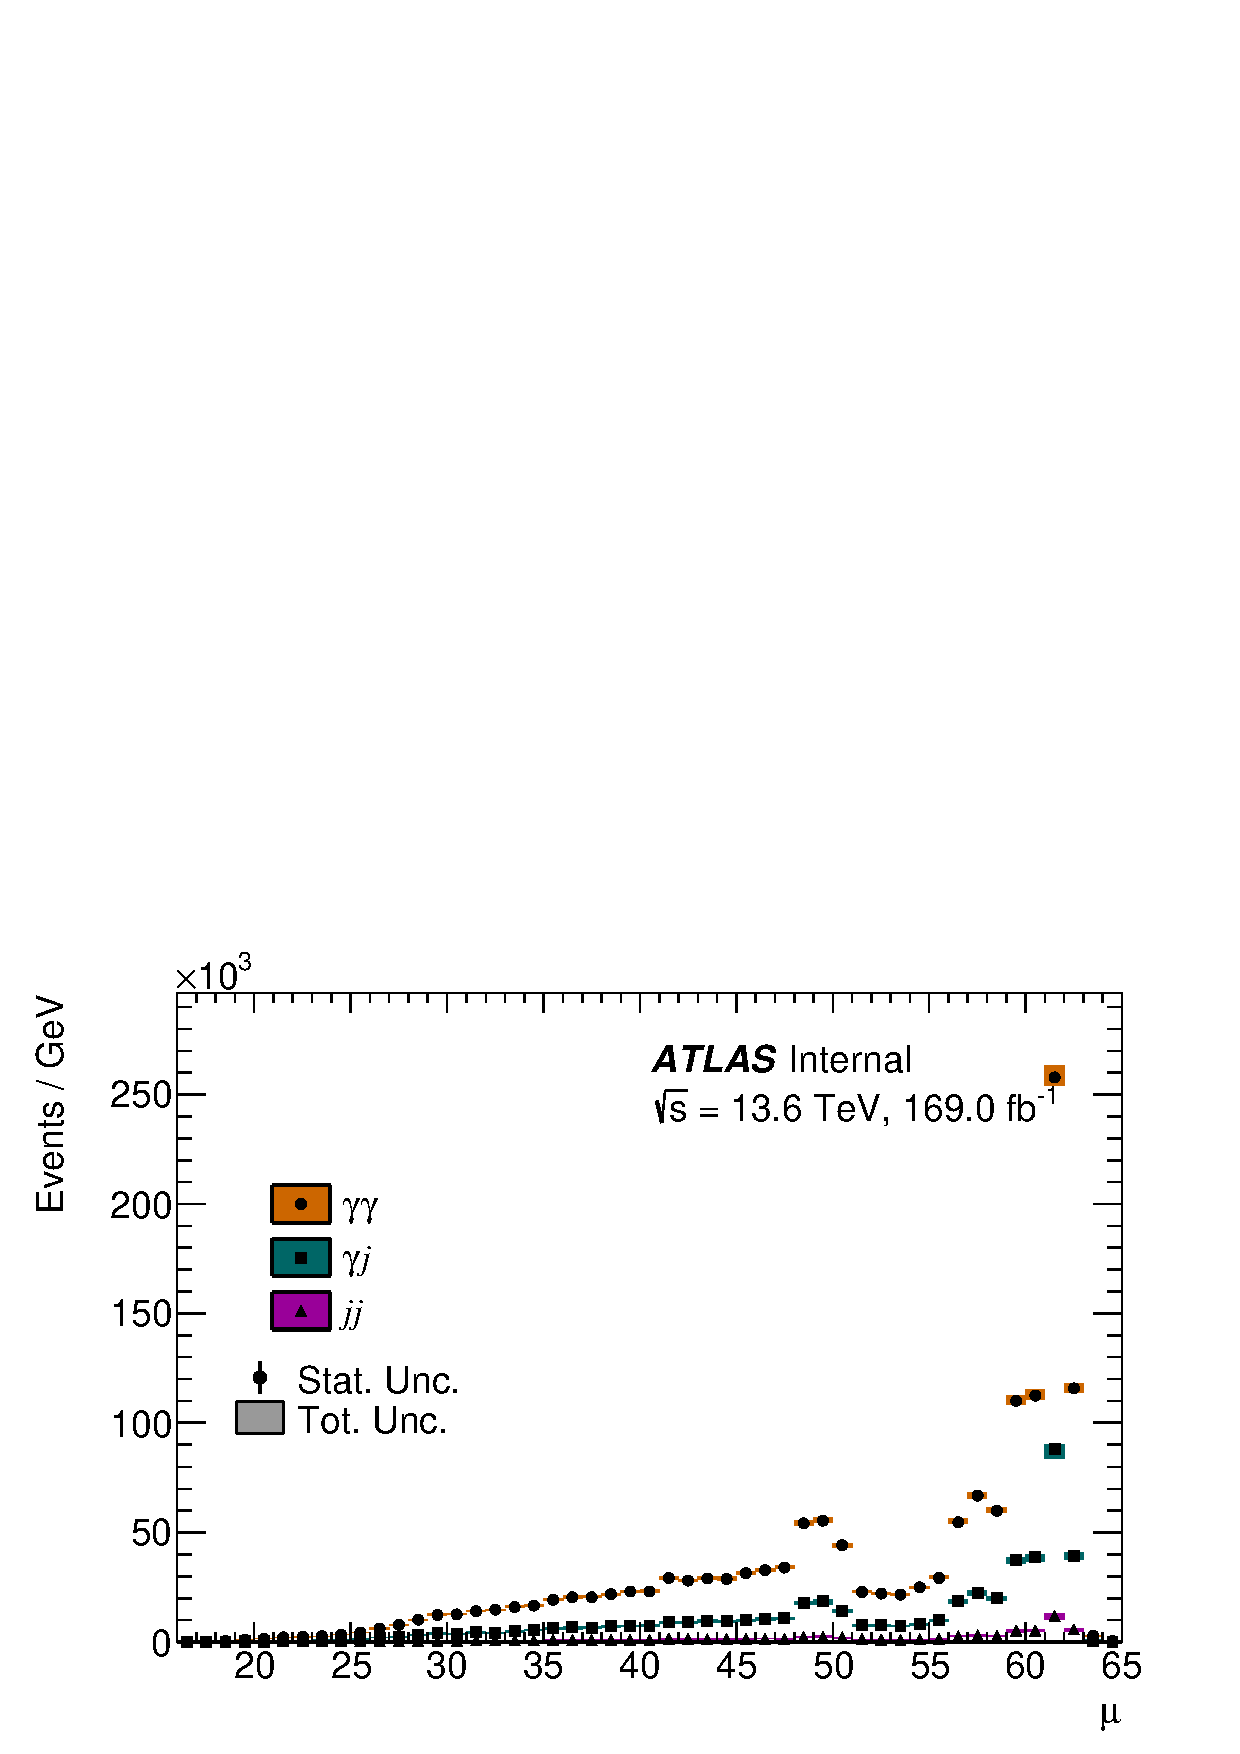
\includegraphics[width=0.8\textwidth]{figures/2x2d_sidebands/plots_sb_diffxsvars_20250930/plot_bkgDecomp_Inclusive_mu.pdf}
    \label{fig:2x2dmu202224}
    \caption{Background yields as a function of $\mu$ for 2022--2024 data (\texttt{mc23a--e}).}
\end{figure}


\begin{figure}[!h]
    \centering
    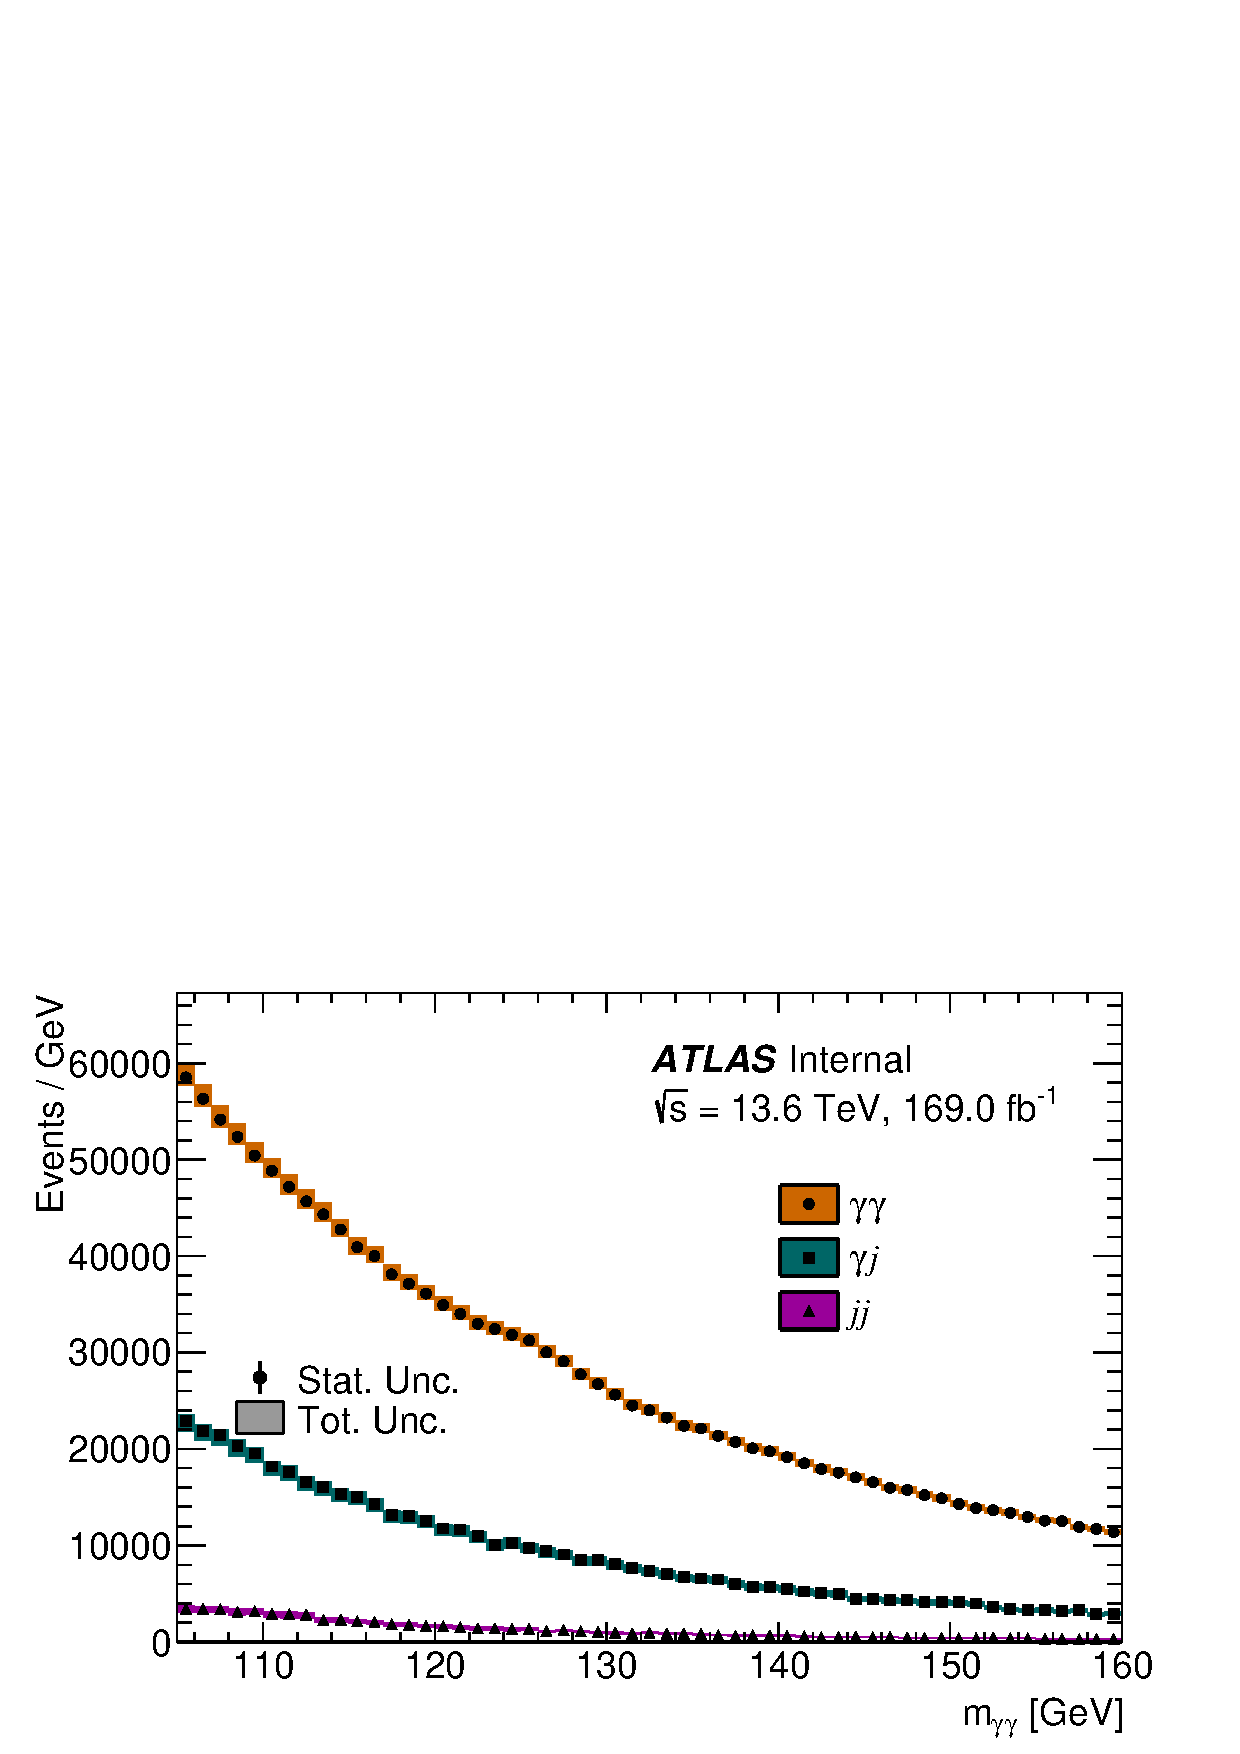
\includegraphics[width=0.8\textwidth]{figures/2x2d_sidebands/plots_sb_diffxsvars_20250930/plot_bkgDecomp_Inclusive_m_yy.pdf}
    \label{fig:2x2dmyy202224}
    \caption{Background yields as a function of $m_{\gamma \gamma}$ for 2022--2024 data (\texttt{mc23a--e}).}
\end{figure}


\begin{figure}[!h]
    \centering
    \includegraphics[width=0.8\textwidth]{figures/2x2d_sidebands/plots_sb_diffxsvars_20250930/plot_bkgDecomp_inclusive_pT_yy.pdf}
    \label{fig:2x2dptyy202224}
    \caption{Background yields as a function of $p_{\mathrm{T}}^{\gamma \gamma}$ for 2022--2024 data (\texttt{mc23a--e}).}
\end{figure}


\begin{figure}[!h]
    \centering
    \includegraphics[width=0.8\textwidth]{figures/2x2d_sidebands/plots_sb_diffxsvars_20250930/plot_bkgDecomp_inclusive_yAbs_yy.pdf}
    \label{fig:2x2dmyabsyy202224}
    \caption{Background yields as a function of $|y_{\gamma \gamma}|$ for 2022--2024 data (\texttt{mc23a--e}).}
\end{figure}


\begin{figure}[!h]
    \centering
    \includegraphics[width=0.8\textwidth]{figures/2x2d_sidebands/plots_sb_diffxsvars_20250930/plot_bkgDecomp_inclusive_pT_j1_30.pdf}
    \label{fig:2x2dptj1202224}
    \caption{Background yields as a function of $p_{\mathrm{T}}^{j_1}$ for 2022--2024 data (\texttt{mc23a--e}).}
\end{figure}


\begin{figure}[!h]
    \centering
    \includegraphics[width=0.8\textwidth]{figures/2x2d_sidebands/plots_sb_diffxsvars_20250930/plot_bkgDecomp_inclusive_N_j_30.pdf}
    \label{fig:2x2dnjets202224}
    \caption{Background yields as a function of $N_{\mathrm{jets}}$ for 2022--2024 data (\texttt{mc23a--e}).}
\end{figure}


\begin{figure}[!h]
    \centering
    \includegraphics[width=0.8\textwidth]{figures/2x2d_sidebands/plots_sb_diffxsvars_20250930/plot_bkgDecomp_inclusive_m_jj_30.pdf}
    \label{fig:2x2dmjj202224}
    \caption{Background yields as a function of $m_{jj}$ for 2022--2024 data (\texttt{mc23a--e}).}
\end{figure}


\begin{figure}[!h]
    \centering
    \includegraphics[width=0.8\textwidth]{figures/2x2d_sidebands/plots_sb_diffxsvars_20250930/plot_bkgDecomp_inclusive_Dphi_j_j_30_signed.pdf}
    \label{fig:2x2ddphijj202224}
    \caption{Background yields as a function of $\Delta \phi_{jj}$ for 2022--2024 data (\texttt{mc23a--e}).}
\end{figure}


\begin{figure}[!h]
    \centering
    \includegraphics[width=0.8\textwidth]{figures/2x2d_sidebands/plots_sb_diffxsvars_20250930/plot_bkgDecomp_inclusive_N_j_btag30.pdf}
    \label{fig:2x2dnbjets202224}
    \caption{Background yields as a function of $N_{\mathrm{b-jets}}$ for 2022--2024 data (\texttt{mc23a--e}).}
\end{figure}


\begin{figure}[!h]
    \centering
    \includegraphics[width=0.8\textwidth]{figures/2x2d_sidebands/plots_sb_diffxsvars_20250930/plot_bkgDecomp_inclusive_N_lep_15.pdf}
    \label{fig:2x2dnlept202224}
    \caption{Background yields as a function of $N_{\mathrm{leptons}}$ for 2022--2024 data (\texttt{mc23a--e}).}
\end{figure}



\newpage
\FloatBarrier

\subsubsection{Differential Plots: Background Fractions}
\label{subsec:2x2dfractionsplots}


\begin{figure}[!h]
    \centering
    \includegraphics[width=0.8\textwidth]{figures/2x2d_sidebands/plots_sb_diffxsvars_20250930/plot_purity_inclusive.pdf}
    \label{fig:2x2dpurinclusive202224}
    \caption{Inclusive background purity for 2022--2024 data (\texttt{mc23a--e}).}
\end{figure}


\begin{figure}[!h]
    \centering
    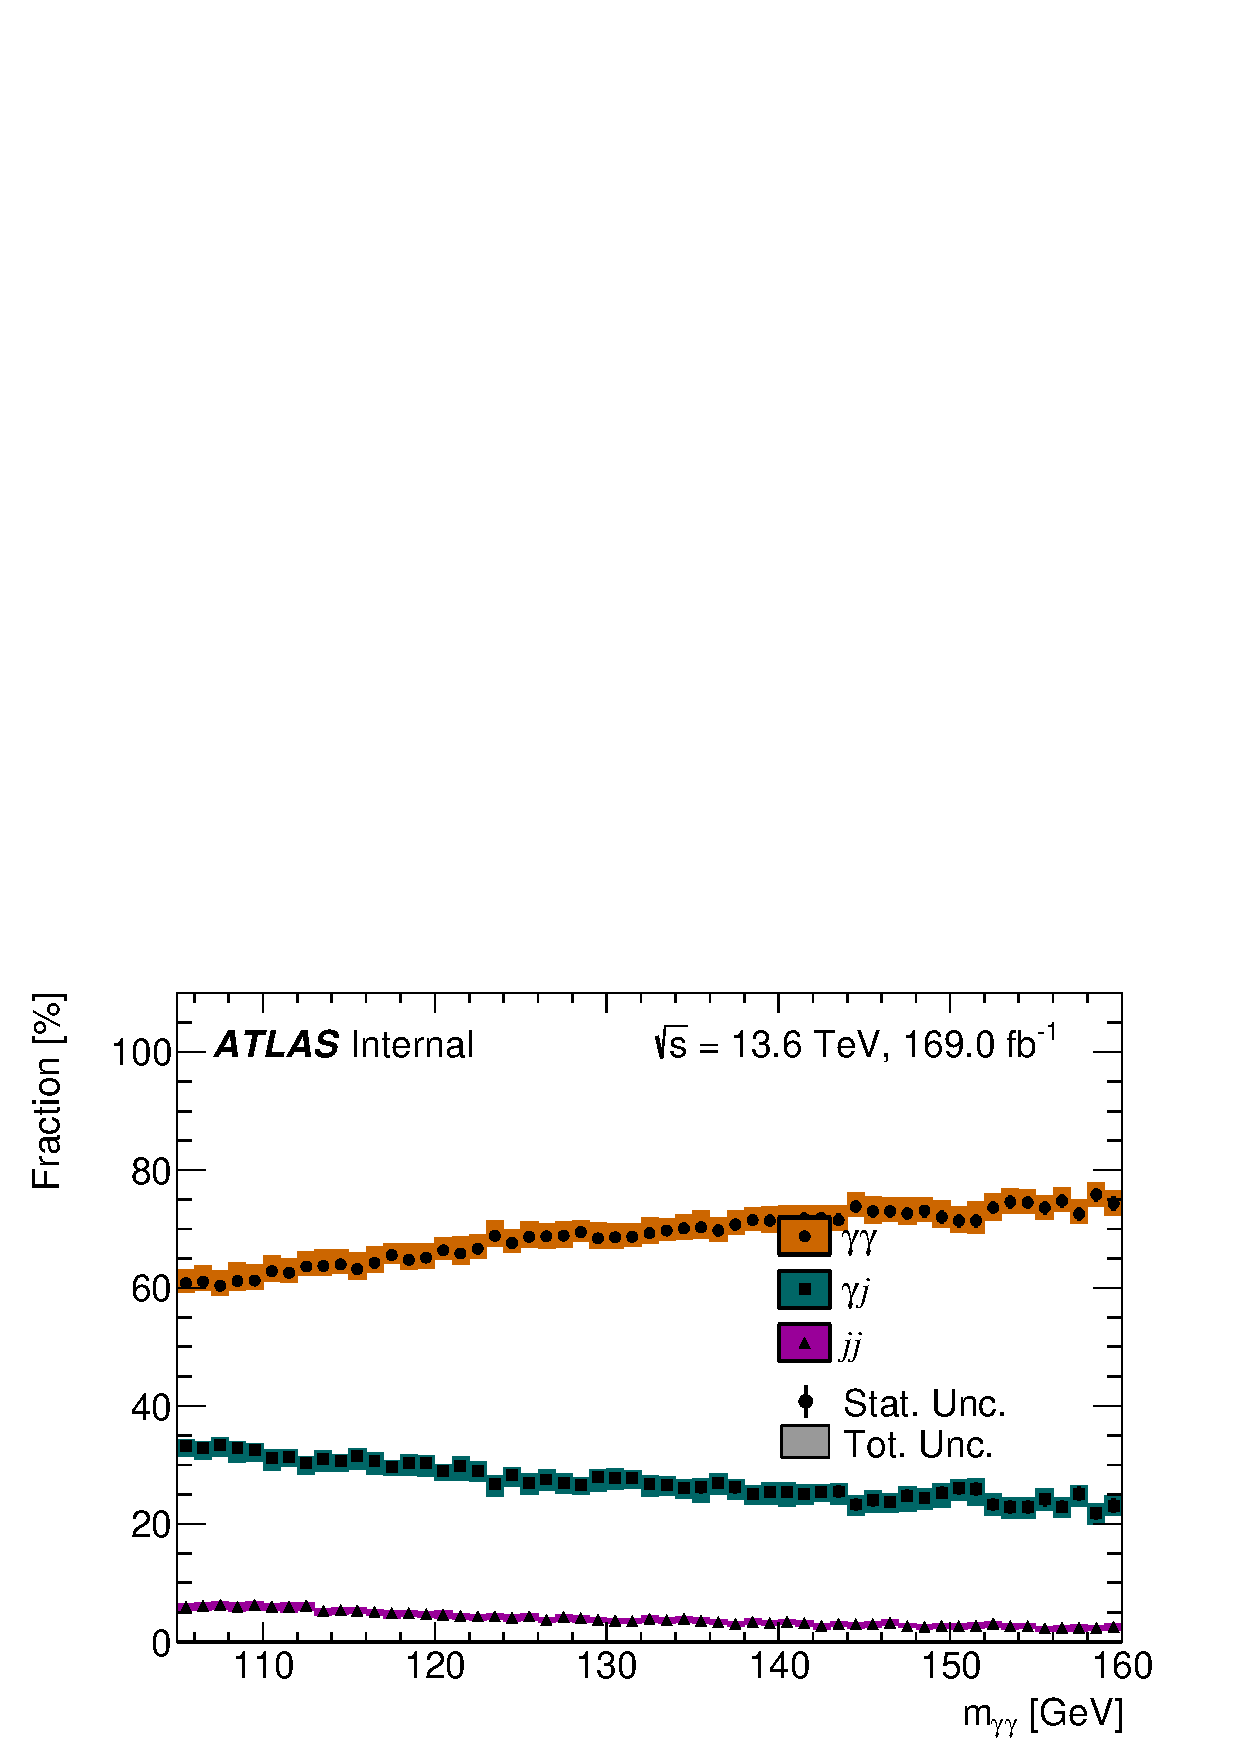
\includegraphics[width=0.8\textwidth]{figures/2x2d_sidebands/plots_sb_diffxsvars_20250930/plot_purity_m_yy.pdf}
    \label{fig:2x2dpurmyy202224}
    \caption{Background purity as a function of $m_{\gamma \gamma}$ for 2022--2024 data (\texttt{mc23a--e}).}
\end{figure}


\begin{figure}[!h]
    \centering
    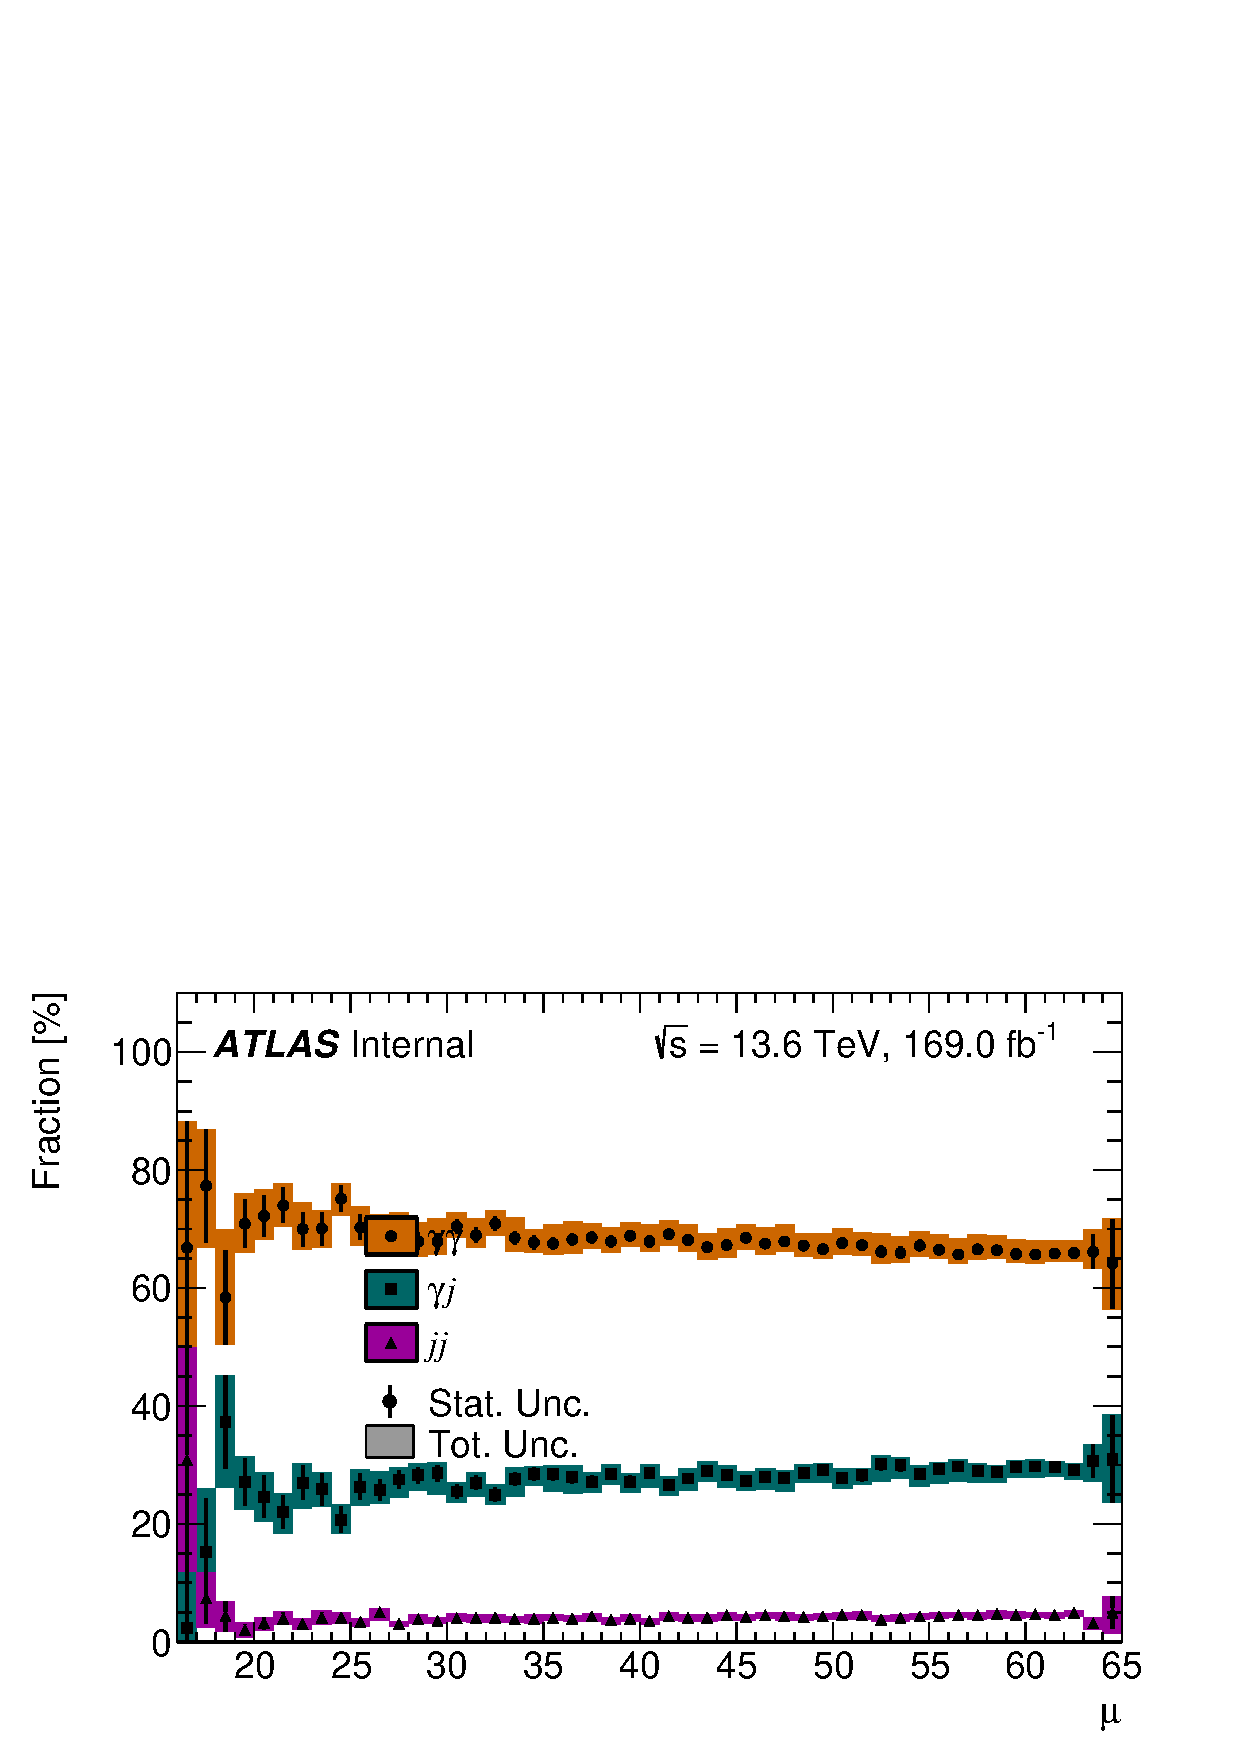
\includegraphics[width=0.8\textwidth]{figures/2x2d_sidebands/plots_sb_diffxsvars_20250930/plot_purity_mu.pdf}
    \label{fig:2x2dpurmu202224}
    \caption{Background purity as a function of $\mu$ for 2022--2024 data (\texttt{mc23a--e}).}
\end{figure}


\begin{figure}[!h]
    \centering
    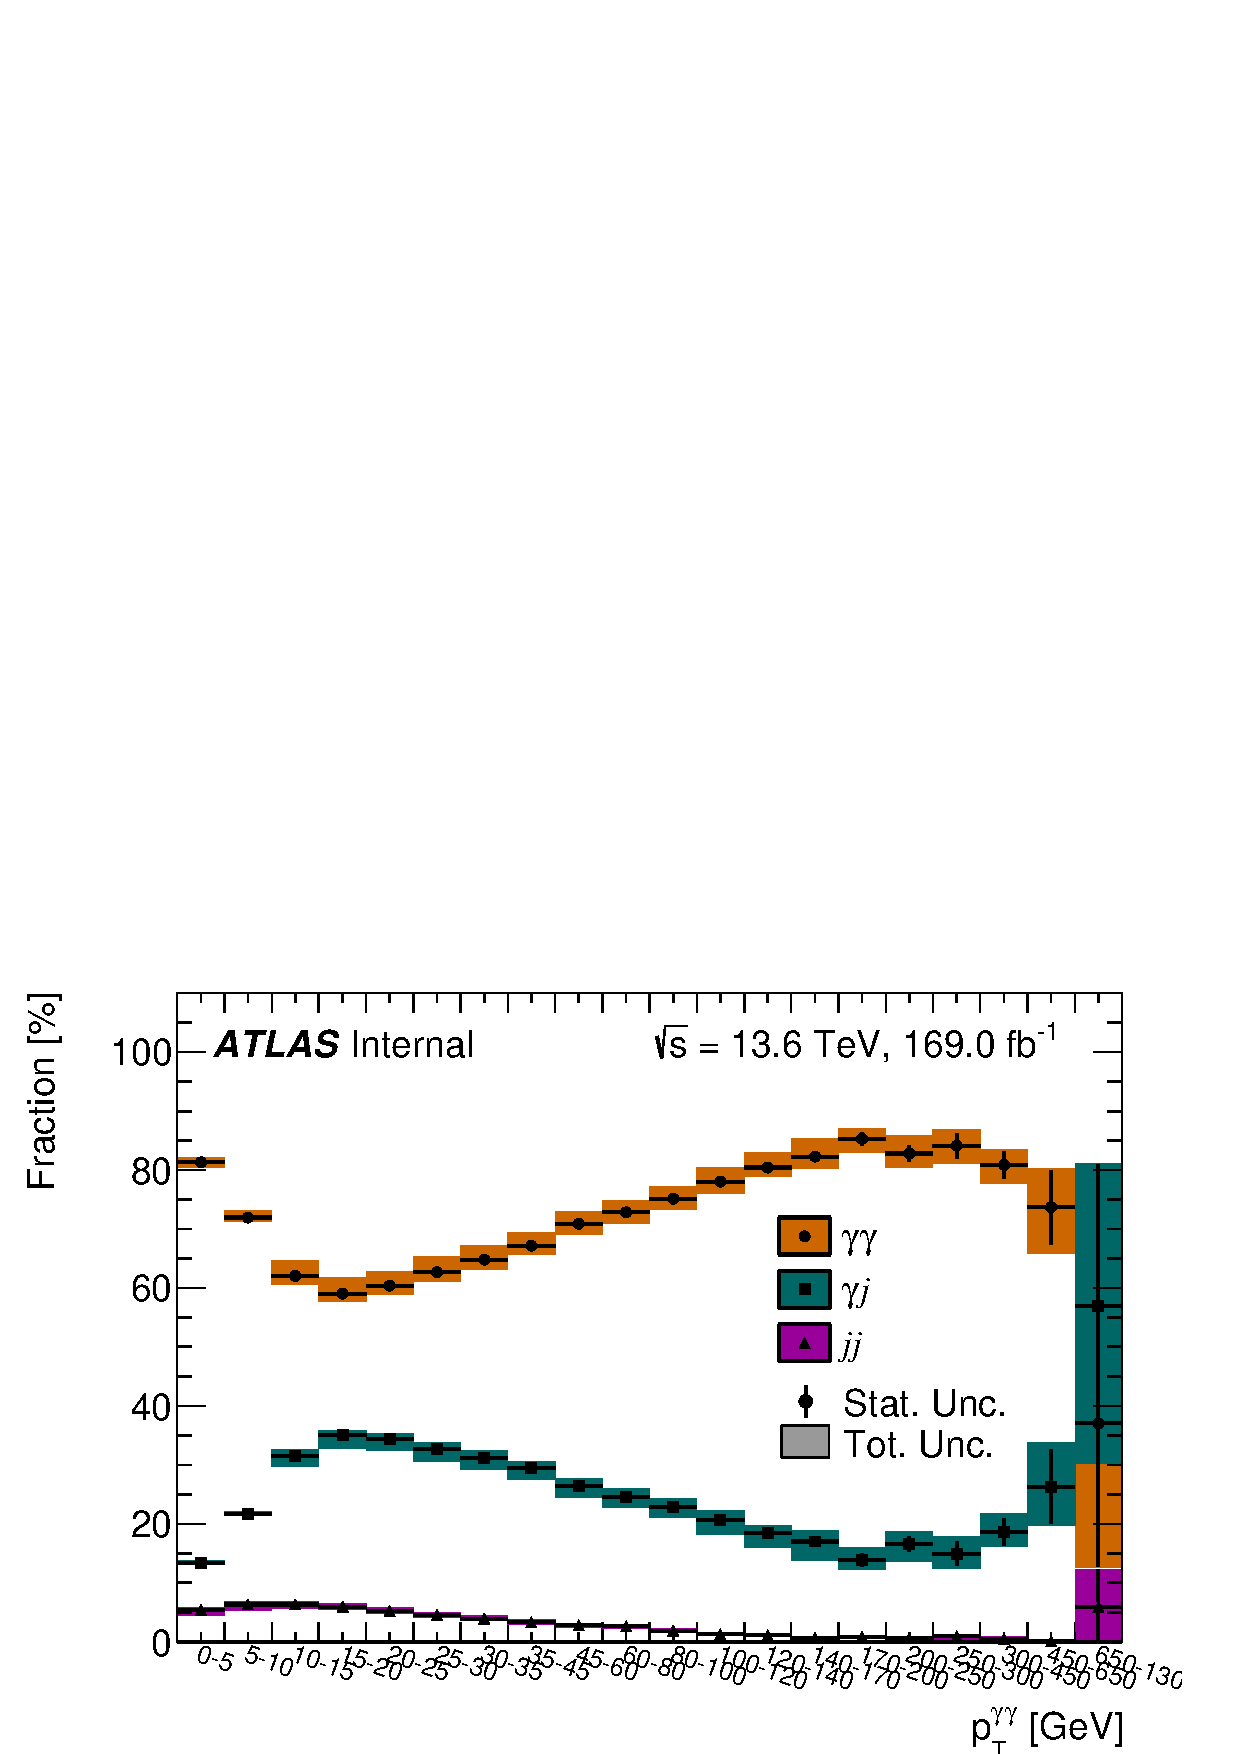
\includegraphics[width=0.8\textwidth]{figures/2x2d_sidebands/plots_sb_diffxsvars_20250930/plot_purity_pT_yy.pdf}
    \label{fig:2x2dpurptyy202224}
    \caption{Background purity as a function of $p_{\mathrm{T}}^{\gamma \gamma}$ for 2022--2024 data (\texttt{mc23a--e}).}
\end{figure}


\begin{figure}[!h]
    \centering
    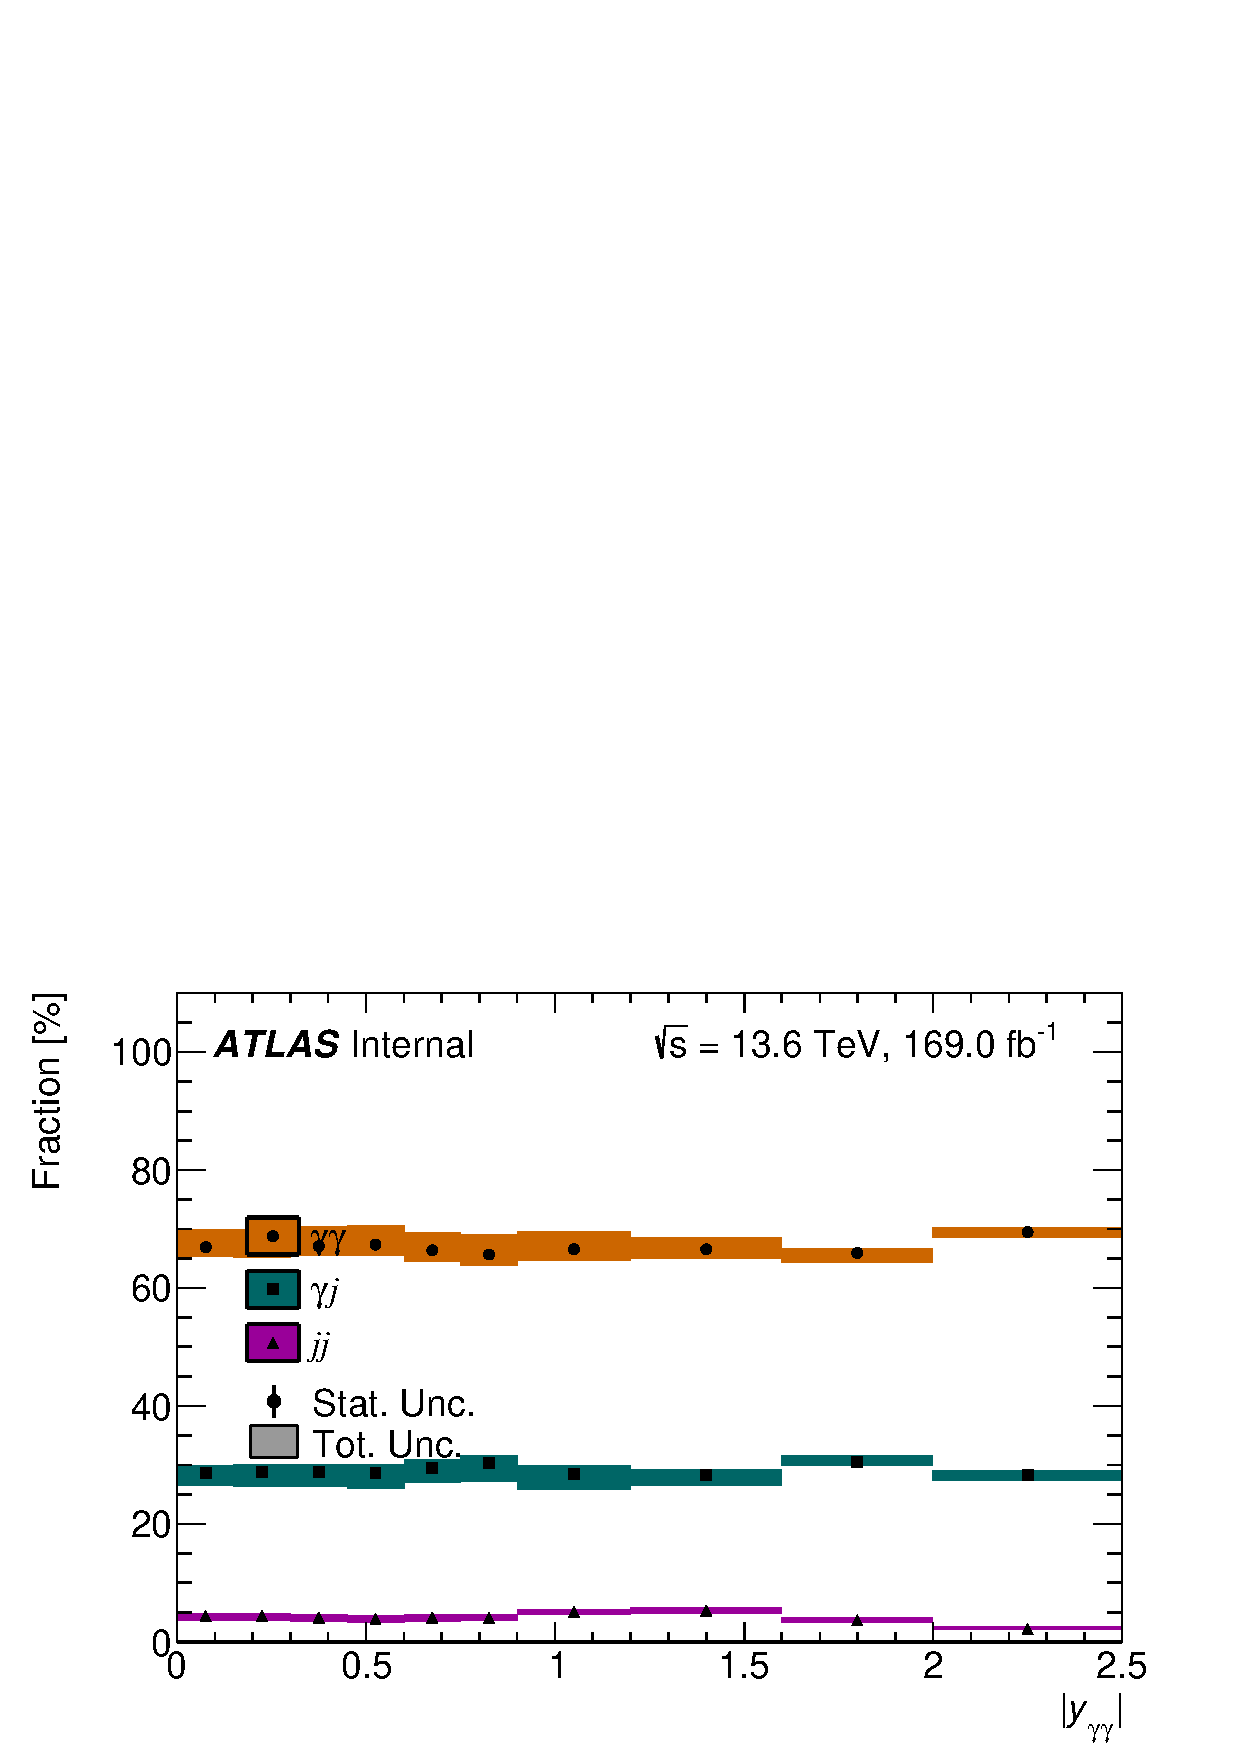
\includegraphics[width=0.8\textwidth]{figures/2x2d_sidebands/plots_sb_diffxsvars_20250930/plot_purity_yAbs_yy.pdf}
    \label{fig:2x2dpuryabsyy202224}
    \caption{Background purity as a function of $|y_{\gamma \gamma}|$ for 2022--2024 data (\texttt{mc23a--e}).}
\end{figure}


\begin{figure}[!h]
    \centering
    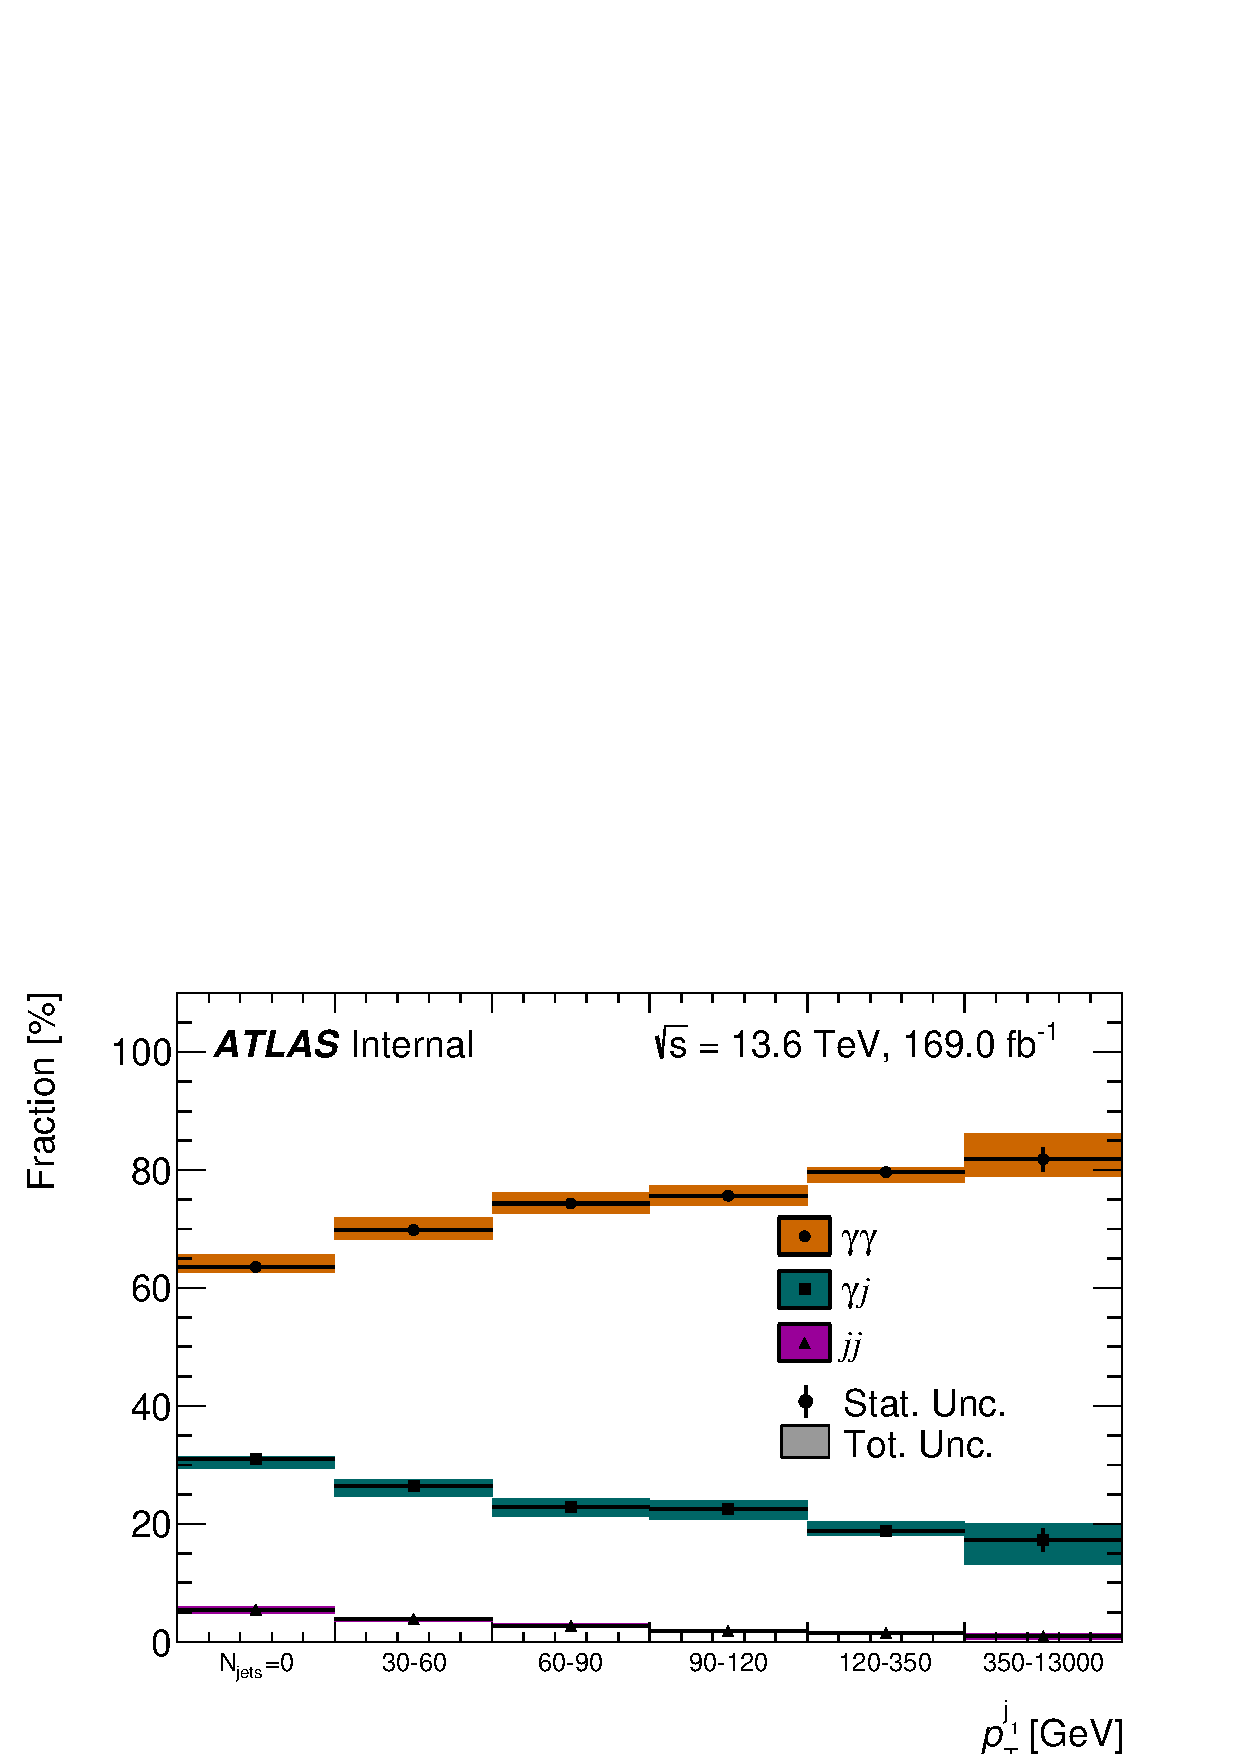
\includegraphics[width=0.8\textwidth]{figures/2x2d_sidebands/plots_sb_diffxsvars_20250930/plot_purity_pT_j1_30.pdf}
    \label{fig:2x2dpurptj1202224}
    \caption{Background purity as a function of $p_{\mathrm{T}}^{j_1}$ for 2022--2024 data (\texttt{mc23a--e}).}
\end{figure}


\begin{figure}[!h]
    \centering
    \includegraphics[width=0.8\textwidth]{figures/2x2d_sidebands/plots_sb_diffxsvars_20250930/plot_purity_N_j_30.pdf}
    \label{fig:2x2dpurnjets202224}
    \caption{Background purity as a function of $N_{\mathrm{jets}}$ for 2022--2024 data (\texttt{mc23a--e}).}
\end{figure}


\begin{figure}[!h]
    \centering
    \includegraphics[width=0.8\textwidth]{figures/2x2d_sidebands/plots_sb_diffxsvars_20250930/plot_purity_m_jj_30.pdf}
    \label{fig:2x2dpurmjj202224}
    \caption{Background purity as a function of $m_{jj}$ for 2022--2024 data (\texttt{mc23a--e}).}
\end{figure}


\begin{figure}[!h]
    \centering
    \includegraphics[width=0.8\textwidth]{figures/2x2d_sidebands/plots_sb_diffxsvars_20250930/plot_purity_Dphi_j_j_30_signed.pdf}
    \label{fig:2x2dpurdphijj202224}
    \caption{Background purity as a function of $\Delta \phi_{jj}$ for 2022--2024 data (\texttt{mc23a--e}).}
\end{figure}


\begin{figure}[!h]
    \centering
    \includegraphics[width=0.8\textwidth]{figures/2x2d_sidebands/plots_sb_diffxsvars_20250930/plot_purity_N_j_btag30.pdf}
    \label{fig:2x2dpurnbjets202224}
    \caption{Background purity as a function of $N_{\mathrm{b-jets}}$ for 2022--2024 data (\texttt{mc23a--e}).}
\end{figure}


\begin{figure}[!h]
    \centering
    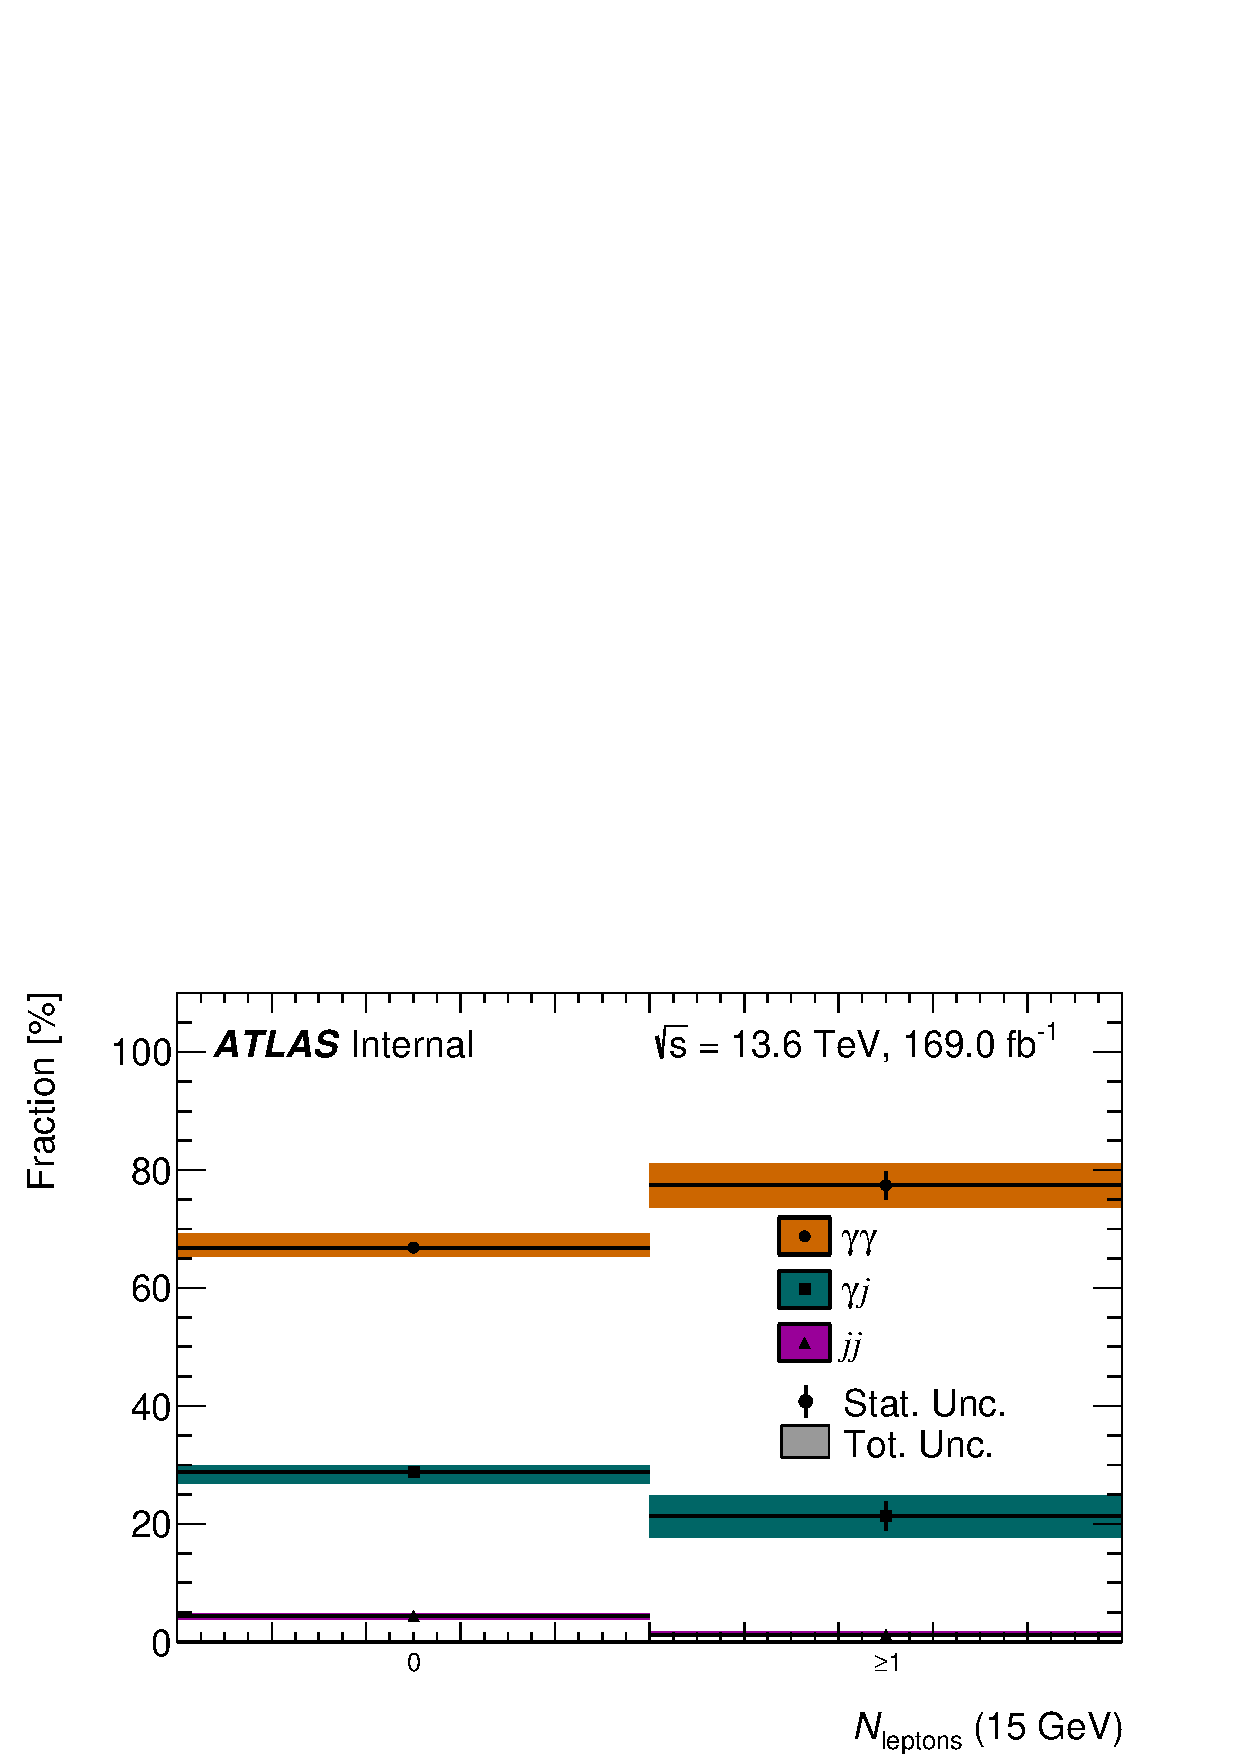
\includegraphics[width=0.8\textwidth]{figures/2x2d_sidebands/plots_sb_diffxsvars_20250930/plot_purity_N_lep_15.pdf}
    \label{fig:2x2dpurnlept202224}
    \caption{Background purity as a function of $N_{\mathrm{leptons}}$ for 2022--2024 data (\texttt{mc23a--e}).}
\end{figure}

